% build with: pdflatex --shell-escape fig.tex
\documentclass[tikz, convert={density=800}]{standalone}

\usepackage{tikz}
\definecolor{myOrange}{HTML}{ffa500}
\definecolor{myBlue}{HTML}{42affa}

\begin{document}
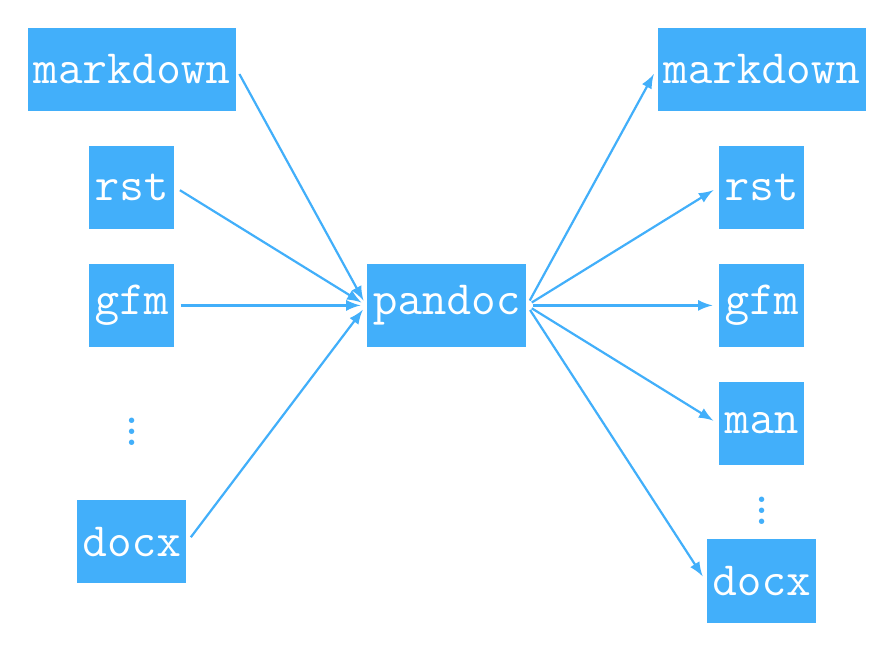
\begin{tikzpicture}[>=latex, thick, shorten >=2pt, shorten <=2pt, ->, myBlue]

%  \tikzstyle{C}=[circle,fill=myBlue,text=white,minimum size=30pt,inner sep=2pt, font=\LARGE]
  \tikzstyle{C}=[rectangle,fill=myBlue,text=white,minimum size=30pt,inner sep=2pt, font=\LARGE]
  \tikzstyle{M}=[circle,fill=myOrange,text=white,minimum size=30pt,inner sep=2pt, font=\LARGE]
  \tikzstyle{B}=[text=myBlue, font=\LARGE]

%  \node[C] at (0,3) (bin) {\texttt{/bin}};
%  \node[C] at (2,3) (sbin) {\texttt{/sbin}};
%  \node[C] at (4,3) (usr) {\texttt{/usr}};
%  \node[C] at (6,3) (lib) {\texttt{/lib}};
%  \node[C] at (8,3) (dots) {\texttt{/home}};
%  \node[C] at (10,3) (dots) {\texttt{\ldots}};
  
%  \node[C] at (6,1) (E) {\texttt{E}};
%  
%  \node[M] at (9,3) (M) {\texttt{M}};

%  \draw [<-] (usr) to (usrbin);
%  \draw [<-] (usr) to (usrlocal);
%  \draw [<-] (usr) to (usrinclude);
%  \draw [<-] (usr) to (usrlib);
%  \draw [<-] (usr) to (usrdots);
%  
%  
%  \draw [<-] (usrlocal) to (usrlocalbin);
%  \draw [<-] (usrlocal) to (usrlocallib);
%  \draw [<-] (usrlocal) to (usrlocalinclude);
%  \draw [<-] (usrlocal) to (usrlocaldots);
  
%  \draw [<-] (A) to (B);
%  \draw [<-] (B) to (C);
%  \draw [<-] (A) to (D);
%  \draw [<-] (D) to (E);
%  \draw [<-, myOrange] (C) to (M);
%  \draw [<-, myOrange] (E) to (M);
  
  \node[C] at (-2,3) (markdown) {\texttt{markdown}};
  \node[C] at (-2,1.5) (rst) {\texttt{rst}};
  \node[C] at (-2,-0.0) (gfm) {\texttt{gfm}};
  \node[B] at (-2,-1.5) (dots) {\texttt{\vdots}};
  \node[C] at (-2,-3.0) (docx) {\texttt{docx}};
  
  
  \node[C] at (2,-0) (pandoc) {\texttt{pandoc}};
  
%  \draw [] (usr.south) to (usrlevel.north);
%  \draw [] (usrlocal) to (usrlocallevel);

  \draw [] (markdown.east) to (pandoc.west);
  \draw [] (rst.east) to (pandoc.west);
  \draw [] (gfm.east) to (pandoc.west);
  \draw [] (docx.east) to (pandoc.west);
  
  \node[C] at (6,3) (markdownR) {\texttt{markdown}};
  \node[C] at (6,1.5) (rstR) {\texttt{rst}};
  \node[C] at (6,-0.) (gfmR) {\texttt{gfm}};
  \node[C] at (6,-1.5) (manR) {\texttt{man}};
  \node[B] at (6,-2.5) (dotsR) {\texttt{\vdots}};
  \node[C] at (6,-3.5) (docxR) {\texttt{docx}};
  
  \draw [] (pandoc.east) to (markdownR.west);
  \draw [] (pandoc.east) to (rstR.west);
  \draw [] (pandoc.east) to (gfmR.west);
  \draw [] (pandoc.east) to (manR.west);
  \draw [] (pandoc.east) to (docxR.west);
  
  
\end{tikzpicture}
\end{document}
